\documentclass{article}
\usepackage{thomaspackage}
\usetikzlibrary{matrix}

\begin{document}
	\tableofcontents
	\newpage

	\section{Limieten}
    Bekende limieten zijn
    \[
        \lim_{x\to 0} \frac{x}{\sin x} = 1
    \]
	\section{Sommen}
 		Onthoud:
 		\begin{align*}
 			\sum_{k=c}^{\infty} r^k &= \frac{r^c}{1-r} \text{ als $|r|<1$}\\
 			\sum_{k=1}^{\infty} \frac{1}{k^2} &= \frac{\pi^2}{6} \\
 			\sum_{k=0}^\infty \frac{x^k}{k!} &= e^x \\
 		\end{align*}
 		
 		Uit de eerste kunnen we andere sommen afleiden. bijvoorbeeld 
 		$\displaystyle \sum_{k=0}^{\infty} kr^k: $
 		\begin{align*}
 				\sum_{k=0}^{\infty} r^k &= \frac{1}{1-r} \text { differenti\"eren aan beide kanten } \to \\
 				\sum_{k=1}^{\infty} kr^{k-1} &= \frac{1}{(1-r)^2} \\
 				\sum_{k=0}^{\infty} kr^k &= \frac{r}{(1-r)^2} \\
 		\end{align*}
 		Op dezelfde manier $\displaystyle \sum_{k=1}^{\infty} \frac{1}{k2^k}$:
 		\begin{align*}
 				\sum_{k=0}^{\infty} r^k &= \frac{1}{1-r} \text { integreren aan beide kanten } \to \\
 				\sum_{k=0}^{\infty} \frac{1}{k+1} r^{k+1} &= -\log_e (1-r) \\
 				\sum_{k-1}^\infty \frac{1}{k} r^k &= \log_e (\frac{1}{1-r})
 		\end{align*}
 		Eindige sommen kunnen we nu ook, \textbf{deze formule geldt algemener voor $r\neq 1$} maar dan is de afleiding natuurlijk anders.
 		\begin{align*}
 			\sum_{k=c}^n r^k &= \sum_{k=c}^\infty r^k - \sum_{k=n}^\infty r^k
 		\end{align*}

\section{Taylorreeksen}

	Onthoud: de cosinus is even (symmetrisch rond $y$-as) en deze heeft even machten, evenzo is de sinus oneven.
	\begin{align*}
		\cos x &\coloneqq \sum_{n=0}^\infty (-1)^n \frac{x^{2n}}{(2n)!} \\
		\sin x &\coloneqq \sum_{n=0}^\infty (-1)^n \frac{x^{2n+1}}{(2n+1)!} \\
		e^x &\coloneqq \sum_{n=0}^\infty \frac{x^n}{n!} \\
		\ln (1+x) &= \sum_{n=0}^\infty (-1)^{n} \frac{x^{n+1}}{n+1} \\
		\arctan x &= \sum_{n=0}^\infty (-1)^n \frac{x^{2n+1}}{2n+1} \\
	\end{align*}


	\subsection{Cosinus en sinus hyperbolicus}
		Merk op dat deze definities gelijk zijn aan de gewone sinus en cosinus maar dan niet alternerend.
		\begin{align*}
			\cosh z &\coloneqq \frac{1}{2} (e^z + e^{-z}) = \sum_{k=0}^\infty \frac{z^{2k}}{(2k)!} = \text{ alle even termen van de e-machtreeks} \\
			\sinh z &\coloneqq \frac{1}{2} (e^z - e^{-z}) = \sum_{k=0}^\infty \frac{z^{2k+1}}{(2k+1)!} = \text{ alle oneven termen van de e-machtreeks}
		\end{align*}
	\subsection{Matrix in e-macht}
		Deze definitie lijkt op de gewone definitie van $e^x$. Als $A$ een matrix, dan geldt
		\[ e^{At} \coloneqq \sum_{k=0}^\infty \frac{A^k t^k}{k!} \]
		Voor $\displaystyle A = \vvec{0 & 1 \\ 1 & 0}$ geldt dan
		\[ e^{At} =
		\vvec{1 + \frac{t^2}{2!} + \frac{t^4}{4!} + \dots & t + \frac{t^3}{3!} + \dots \\
			t + \frac{t^3}{3!} + \dots & 1 + \frac{t^2}{2!} + \frac{t^4}{4!} + \dots}
		= \vvec{\cosh t & \sinh t \\ \sinh t & \cosh t}\]

	\subsection{Imaginaire e-macht}

	\begin{align*}
		e^{ix} &= \cos x + i \sin x \\
		e^{-ix} &= \sin x + i \cos x
	\end{align*}
 		
 	\section{Integralen}

		\begin{stelling}[Bell curve]
			\[ \int_{-\infty}^\infty e^{-x^2} \d x = \sqrt \pi .\]
		\end{stelling}

	 	\begin{stelling}[Limiet door de integraal halen]
		 	Zij $\f_k,\f \: \reals^n \to \reals$, met $\lim_{k \to \infty} \f_k = \f$, dan
		 	\[ \f_k \text { \textbf{convergeert uniform} naar } \f \implies \lim \int \f_k = \int \lim \f_k = \int \f \,. \]
	 	\end{stelling}
	 	
	\section{Integreren}
        Onthoud:
        \begin{align*}
            \int \frac{1}{\sin^2 u} \d u = \cotan u = \frac{1}{\tan u}
        \end{align*}
        \subsection{Partieel integreren}
            \[
                \int_a^b f(x) g'(x) \d x = \big[f(x)g(x)\big]_a^b - \int_a^b f'(x) g(x) \d x
             \]
             dus kies $f$ en $g$ zodanig dat $f'(x)g(x)$ makkelijk integreert.

        \subsection{Integreren door twee keer partieel}
            Als je een integraal van bijvoorbeeld de vorm
            \[
                \int \sin t \cdot e^t \d t
            \]
            hebt, kun je opmerken dat als je een sinus twee keer integreert je weer een sinus
            krijgt, en dus weer dezelfde integraal. Dit kunnen we toepassen
            door twee keer partieel te integreren (grenzen weggelaten voor de duidelijkheid).
            \begin{align*}
                \int \sin t \cdot e^t \d t &= \sin t \cdot e^t - \int \cos t \cdot e^t \d t
                \quad \text{ met $f=\sin t$ en $g'=e^t$} \\
                &= \sin t \cdot e^t - \left( \cos t \cdot e^t - \int - \sin t \cdot e^t \d t \right)
                \quad \text{ met $f=\cos t$ en $g'=e^t$} \\
                &= ( \sin t - \cos t ) e^t -  \int \sin t \cdot e^t \d t
            \end{align*}
            Hieruit volgt dat
            \[  \int \sin t \cdot e^t \d t = \frac{1}{2} ( \sin t - \cos t ) e^t\,. \]

        \subsection{Integreren door breuksplitsen}
            We bekijken
            \begin{align*}
                \int \frac{1}{u(1-u)} \d u &= \int \frac{A}{u} + \frac{B}{1-u} \d u \\
                &= \int \frac{A(1-u)+Bu}{u(1-u)} \d u
            \end{align*}
            waaruit volgt $A=B=1$ en dus
            \[ \int \frac{1}{u(1-u)} \d u = \ln |u| + \ln |1-u|\,. \]
        \subsection{Integreren door substitutie}
            We bekijken
            \[ \int \sin t \cdot \cos t \cdot e^{\sin t} \d t\,. \]
            Hierin zou je een functie en zijn afgeleide kunnen herkennen, namelijk
            $\sin t$ en $\cos t$ waarbij een eventuele factor natuurlijk niet uitmaakt.
            We substitueren $u = \sin t$, waaruit volgt $\d u = \cos t \d t$
            zodat de integraal overgaat in
            \[ \int u e^u \d u \]
            wat we kunnen uitrekenen met partieel integeren. Er volgt
            \begin{align*}
                \int u e^u \d u &= u e^u - \int e^u \d u \\
                &=  u e^u -  e^u + c \\
                &= (\sin t -1) e^{\sin t} \,.
            \end{align*}
            Mochten er grenzen zijn, bijvoorbeeld
            \[ \int_0^{\frac{\pi}{2}} \sin t \cdot \cos t \cdot e^{\sin t} \d t\,. \]
            dan moeten we deze grenzen meesubstitueren, dus
            \[ \int_{\sin 0}^{\sin \frac{\pi}{2}} u e^u \d u = 1\,. \]

	 \section{Gonioformules}
		 Onthoud:
 		 \begin{align*}
 			 \cos (2\alpha) &= \cos^2 \alpha - \sin^2 \alpha \\
 			 \sin (2\alpha) &= 2 \cos \alpha \sin \alpha
 		 \end{align*}
 		 
 		 Mocht je iets willen integreren met $\cos^2$ dan volgt uit de eerste regel
 		 \begin{align*}
 		 		 \cos (2\alpha) &= \cos^2 \alpha - \sin^2 \alpha \\
 		 		 &=  \cos^2 \alpha + \cos^2 \alpha - \cos^2 \alpha - \sin^2 \alpha \\
 		 		 &= 2\cos^2 \alpha -1
 		 	 \end{align*}
 		 	 en evenzo voor $\sin^2$.
	 \section{Co\"ordinaten}
		 Bij cilindercoordinaten is een extra \textbf{factor $\bm r$} verplicht als je integreert, bij bolcoordinaten $\rho^2 \sin \phi$
		 
		 Om bolco\"ordinaten te onthouden, gebruik poolco\"ordinaten en druk $r$ uit in $\rho$ en $\phi$ met behulp van onderstaand driehoekje, zodat $r=\rho \sin \phi$, en vul deze in, in poolco\"ordinaten $r \cos \theta,r \sin \theta$ om $x$ en $y$ te krijgen. Vind de $z$-co\"ordinaat op dezelfde manier zodat $z=\rho \cos \phi$.
		 					
		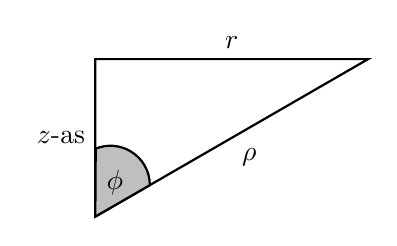
\begin{tikzpicture}[thick]
		\draw(0,0) 
		-- (90:2cm) node[midway,left]{$z$-as} 
		-- (30:4cm) node[midway,above]{$r$} % node of point
		-- (0,0) node[midway,below right]{$\rho$};
		\draw[fill=lightgray, thick] (0,0) 
		-- (30:0.8cm) arc (0:112:0.5cm) node at (60:0.5cm) {$\phi$} 
-- cycle;
		
		\end{tikzpicture}

	\section{Determinant}

		\[
			\det{
				a & b & c \\
				d & e & f \\
				g & h & i \\
			}
			= a \det{e & f \\ h & i} - b \det{d & f \\ g & i} + c \det{d & e \\ g & h}
		\]
		\textbf{Let op het minteken!} Mintekens gaan als volgt:
		\[
			\det{
				+ & - & + \\
				- & + & - \\
				+ & - & +
			}
		 \]
	\section{Inproduct/uitproduct}
		\paragraph{Inproduct (dot product)}
		\[ \x \bullet \bm \phi = \vvec{x \\ y \\ z} \bullet \vvec{\phi_1 \\ \phi_2 \\\phi_3} = x \phi_1 + y \phi_2 + z \phi_3 \]
		\paragraph{Uitproduct (Vector/Cross product)}
		\[ \vvec{x \\ y \\ z} \times \vvec{\phi_1 \\ \phi_2 \\\phi_3} = \vvec{y \phi_3 - \phi_2 z \\ z \phi_1 - \phi_3 x \\ x \phi_2 - \phi_1 y}  \]
		eventueel te onthouden door (zie \LaTeX\ comments)

		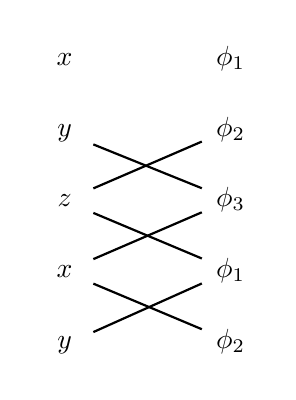
\begin{tikzpicture}[thick]
		\matrix (m) [matrix of math nodes, row sep = 1em, column sep = 4 em, minimum width=2em]
		{
			x & \phi_1 \\
			y & \phi_2 \\
			z & \phi_3 \\
			x & \phi_1 \\
			y & \phi_2 \\
		};
		\path[-stealth]
			(m-2-1) edge[-] (m-3-2) % y keer phi_3
			(m-2-2) edge[-] (m-3-1) % min phi_2 keer z,
			(m-3-1) edge[-] (m-4-2) % z keer phi_1
			(m-3-2) edge[-] (m-4-1) % min phi_3 keer x,
			(m-4-1) edge[-] (m-5-2) % x keer phi_2
			(m-4-2) edge[-] (m-5-1) % min phi_1 keer y
			;
		\end{tikzpicture}
	\section{Bol}
		Inhoud is $\frac{4}{3} \pi r^3$, neem afgeleide voor oppervlakte.

    \section{Tussenwaarde/middelwaardestelling}
    \begin{stelling}[\indx{Tussenwaardestelling}/Intermediate Value Theorem]

        Zij $a,b \in \reals,\ a<b,\
            f:[a,b]\to \reals \text{ continu}\,.
        $
        Zij $f(a)<y<f(b)$. Dan \[ \exists_{c\in(a,b)}:f(c)=y . \]
    \end{stelling}

    \begin{stelling}[\indx{Middelwaardestelling}/Mean Value Theorem]

        Zij $f\:[a,b] \to \reals$ continu, $f|_{(a,b)}$ differentieerbaar. Dan
        \[
        \exists_{c \in (a,b)} : f'(c) = \frac{f(b)-b(a)}{b-a}\,.
        \]
    \end{stelling}
		
	\section{Kwadraat afsplitsen}
        Om een kwadratische vergelijking $x^2 + ax + b = 0$ op te lossen voor $x$ kunnen we in plaats van de abc-formule ook kwadraat afsplitsen. Let wel op dat de co\"efficient voor de $x^2$ een 1 is.
        \begin{align*}
            x^2 + a x + b &= 0 \\
            \left(x + \frac{1}{2} a\right)^2 - \left( \frac{1}{2}a \right)^2 &= - b \\
            \left(x + \frac{1}{2} a\right)^2 &= \left( \frac{1}{2}a \right)^2 - b \\
            x + \frac{1}{2} a &= \pm \sqrt{\left( \frac{1}{2}a \right)^2 - b} \\
            x &= -  \frac{1}{2} a \pm \sqrt{\left(\frac{1}{2}a \right)^2 - b}
        \end{align*}
\end{document}